\documentclass[12pt, oneside, a4paper]{article}
\usepackage{ifpdf}
\usepackage{graphicx}
\usepackage[colorlinks,bookmarksopen,linkcolor=black,pdfauthor={Sharad,Prabhakar,Vikram},urlcolor=blue]{hyperref}
\usepackage[colorlinks,bookmarksopen]{hyperref}
\begin{document}
\begin{center}
\textbf{VISVESWARAYA TECHNOLOGICAL UNIVERSITY}
\end{center}
\begin{center}
\textbf{BELGAUM}\\
\thispagestyle{empty}
\begin{figure}[htb]
\begin{center}
\ifpdf
	
\includegraphics[scale=0.50]{./images/vtu.png}
\else
%	
\includegraphics[scale=0.50]{vtu.png}
\fi
\end{center}
\end{figure}
\textbf{SRI JAYACHAMARAJENDRA COLLEGE OF ENGINEERING}
\textbf{MYSORE-570006}\\
\textsc{department of computer science and engineering}
\end{center}
\begin{figure}[htb]
\begin{center}
\ifpdf

\includegraphics[scale=0.30]{./images/logo.png}
\else
%	
\includegraphics[scale=0.30]{/home/prabhakar/logo.odg}
\fi
\end{center}
\end{figure}
\begin{center}
\textbf{\underline{Project on}}\\
\textsc{MINIMUM VARIANCE HUFFMAN CODING\\}
\emph{\\Under the Guidance of}\\
\textbf{Smt.Trishiladevi C Nagavi}\\
\textit{Senior Scale Lecturer}\\
\textit{Dept of CS$\&$E,SJCE Mysore.}\\
\end{center}
Team:
\begin{center}
\begin{tabular}{|c|c|c|}
\hline
%% row 1
\textsc{name}
&\textsc{roll no}
&\textsc{usn}
\\\hline
%% row 2
\textsc{sharad d}
&03
&\textsc{4jc06cs089}
\\\hline
%% row 3
\textsc{vikram tv}
&61
&\textsc{4jc07cs120}
\\\hline
%% row 4
\textsc{praveen kumar}
&39
&\textsc{4jc07cs073}
\\\hline
%% row 5
\textsc{ravishankar mu}
&47
&\textsc{4jc07cs090}
\\\hline
\end{tabular}
\end{center}
\newpage
\thispagestyle{empty}
\tableofcontents
\newpage
\pagenumbering{arabic}
\section{Introduction}
 The Huffman Coding technique was developed by David Huffman as a part of class assignment.
The codes generated using this technique are called Huffman Codes.
These codes are prefix codes and are optimum for a given model.

The Huffman procedure is based on two observations regarding optimum prefix codes.
\begin{enumerate}
 \item In an optimum code,symbols that occur more frequently(have a higher probability of occurence)will have shorter codewords than symbols that occur less frequently.
\item In an optimum code,the two symbols that occur least frequently will have the same length.
\end{enumerate}

\section{Requirements}
\subsection{Input Requirements}
The input to the program should be given through a file.
The input is a large text files which contains many repeated and non repeated sequence of characters or sentences.

\subsection{Output  Requirements}
 The output of the minimum variance huffman coding is a compressed text file which requires less number of bits to represent them.
\subsection{Functional Requirements}
The program should accept a large text file consisting of many repeated and non repeated sequence of characters or sentences.
It should be effectively able to compress the text file.
\subsection{Nonfunctional Requirements}
\begin{enumerate}
\item Easy to use User interface.
\item Efficiency in analyzing.
\item Versatility in handling all types of  text files.
\item Output suited to be provided for other tool as input.
\end{enumerate}

\subsection{Hardware Requirements}
Minimum Requirements:
\begin{enumerate}
\item 1.1 GHz processor
\item 256 MB RAM or Higher
\item 4GB hard disk
\end{enumerate}
\subsection{Software Requirements}
\begin{enumerate}
\item Linux OS
\item Text Editor 
\item GNU C compiler (gcc)
\item make
\item dotty
\end{enumerate}

\section{Design and Implementation}
 \textbf{\underline{Minimum Variance Huffman Code Design}}\\
 Procedure: 
\begin{enumerate}
 \item Sort the probability of all source symbols in a descending order. 
\item Merge the last two into a new symbol, add their probabilities. 
\item Put the combined symbol as high as possible in the sorted list 
\item Repeat Step 1, 2,3 until only one symbol (the root) is left. 
\item \textbf{Code assignment:}
    Traverse the tree from the root to each leaf node, 
    assign 0 to the left branch and 1 to the right branch. 
\item Compute average codeword length
\end{enumerate}

\subsection{Compression}
  The frequency of each character is counted.  Using the frequency count, a Minimum Variance Huffmann tree is constructed.   A stack is used that contains the frequency of all ascii characters.  An insertion sort is performed on the stack to arrange all the frequencies in non-decreasing order.  The least two frequency count is got from the stack and a binary tree is constructed.  The stack contents are decreased.  The stack is then inserted with the new value of the combined binary tree and reordered.  The construction of the least two frequencies' binary tree is continued until we are left with one node.  The binary tree that gets constructed is attached to its parent.

A dictionary containing the codewords for each character is generated by traversing the minimum variance huffmann tree.  On traversing to the left child, we assign a bit value '0' and on traversing to the right we assign a bit value 1.  The dictionary contains both the character and its appropriate codeword.  Then the dictionary is printed onto a file.

Compression is now performed by referring to the dictionary.  Each character in the input file is read and assigned with a corresponding codeword.  The conversion from bytes to bits is necessary as storing in bytes would expand the input file.  Hence all byte values in compressed file are converted to bit values and stored.  In case of last bit values, zeroes are padded.  Finally, the compression ratio is calculated.  Both the compressed file and the dictionary is sent.

\subsection{Decompression}
 In order to decompress a file, the dictionary contents are read and written into a dictionary structure that contains both the character and the corresponding codeword.  The compressed file is read bit by bit and matched with the codewords.  On a successful match, we decode the bits into the corresponding character and write to the target file.
\section{Screen Shots}
These are the screen shots:\\
\begin{figure}[htb]
\begin{center}
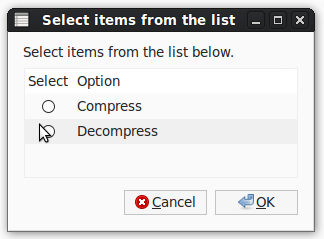
\includegraphics[scale=0.350]{./images/1choice.png}
\end{center}
\caption{Select Compression or Decompression}
\end{figure}

\begin{figure}[htb]
\begin{center}
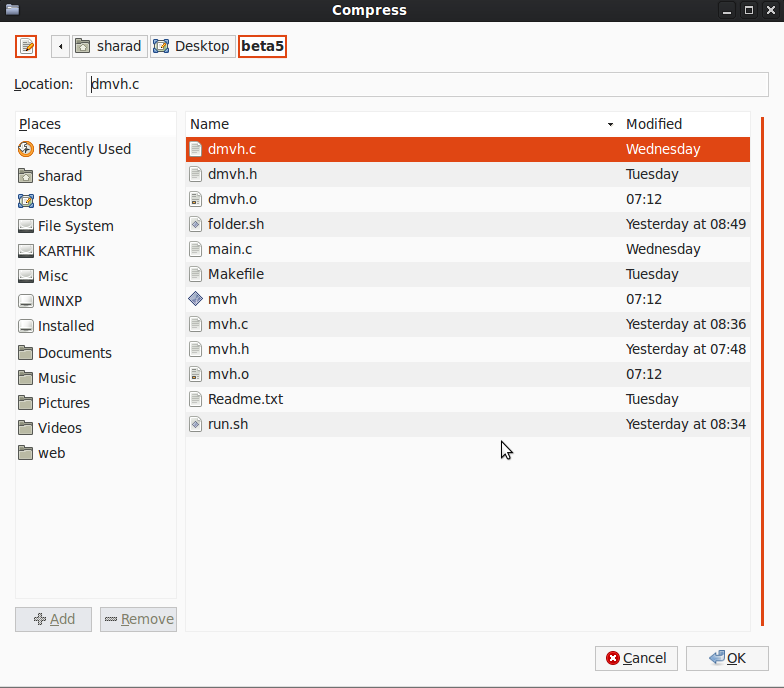
\includegraphics[scale=0.30]{./images/2compsrc.png}
\end{center}
\caption{Select Compression Source}
\end{figure}

\begin{figure}[htb]
\begin{center}
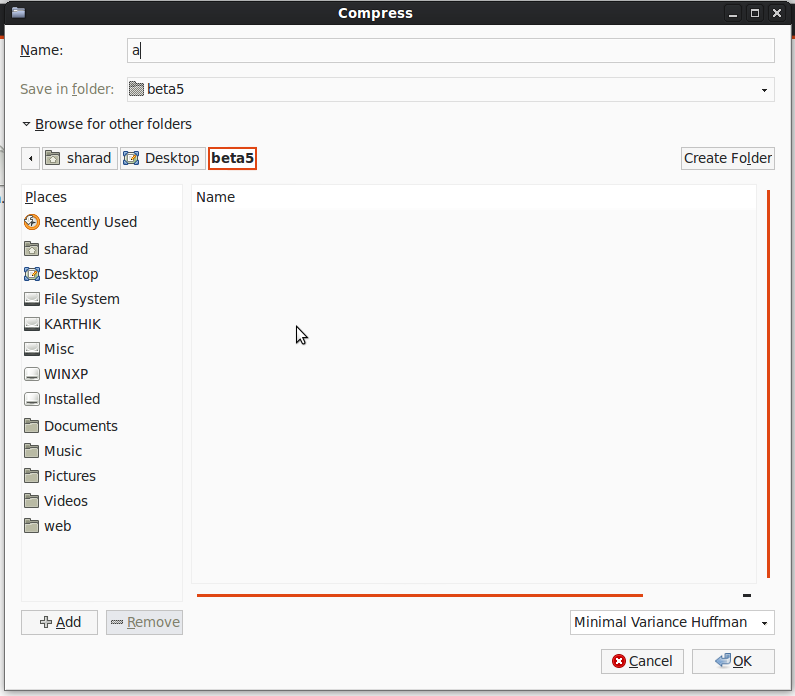
\includegraphics[scale=0.350]{./images/3savecomp.png}
\end{center}
\caption{Select Compression Destination}
\end{figure}

\begin{figure}[htb]
\begin{center}
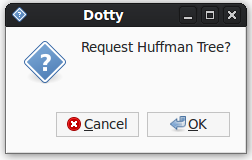
\includegraphics[scale=0.60]{./images/4reqdotty.png}
\caption{Request for Huffmann tree}
\end{center}
\end{figure}

\begin{figure}[htb]
\begin{center}
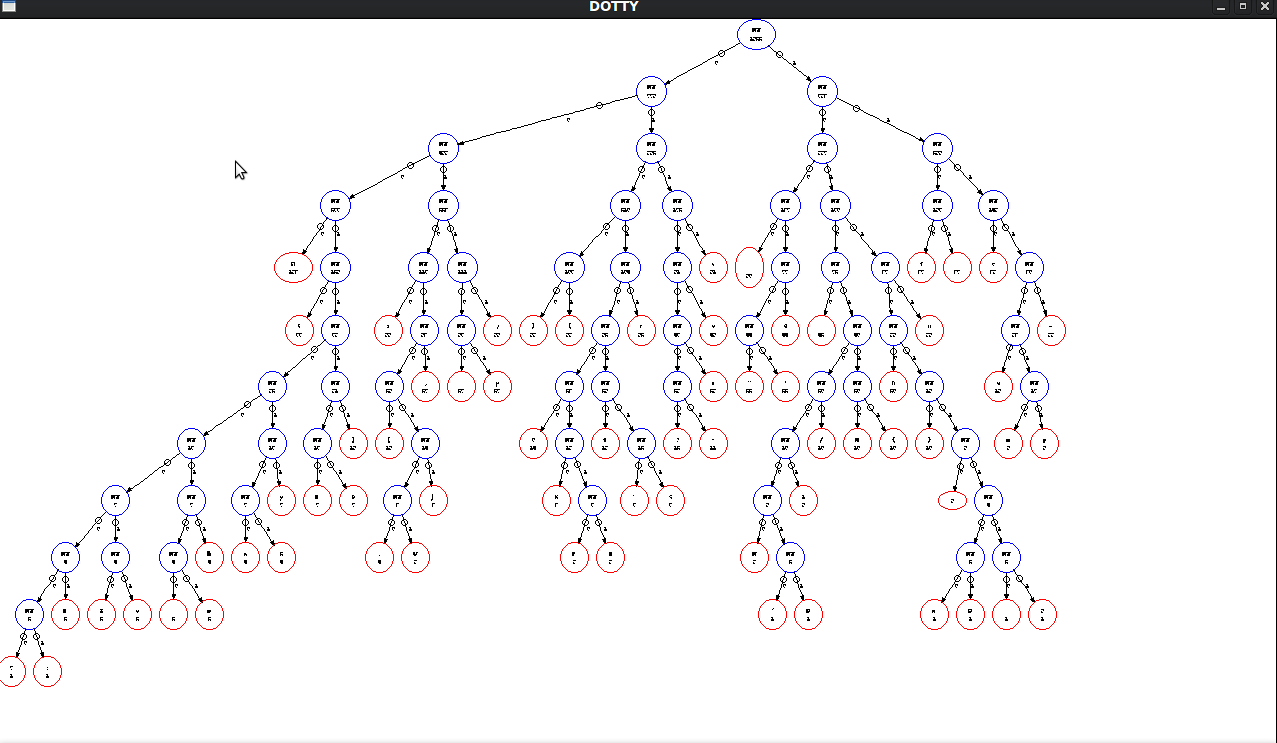
\includegraphics[scale=0.250]{./images/5dotty.png}
\end{center}
\caption{Dotty Display}
\end{figure}

\begin{figure}[htb]
\begin{center}
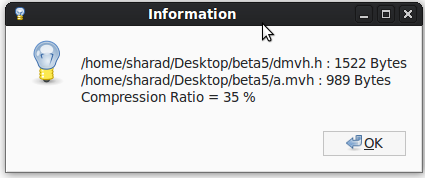
\includegraphics[scale=0.50]{./images/6info.png}
\end{center}
\caption{Show Compression Ratio}
\end{figure}


\begin{figure}[htb]
\begin{center}
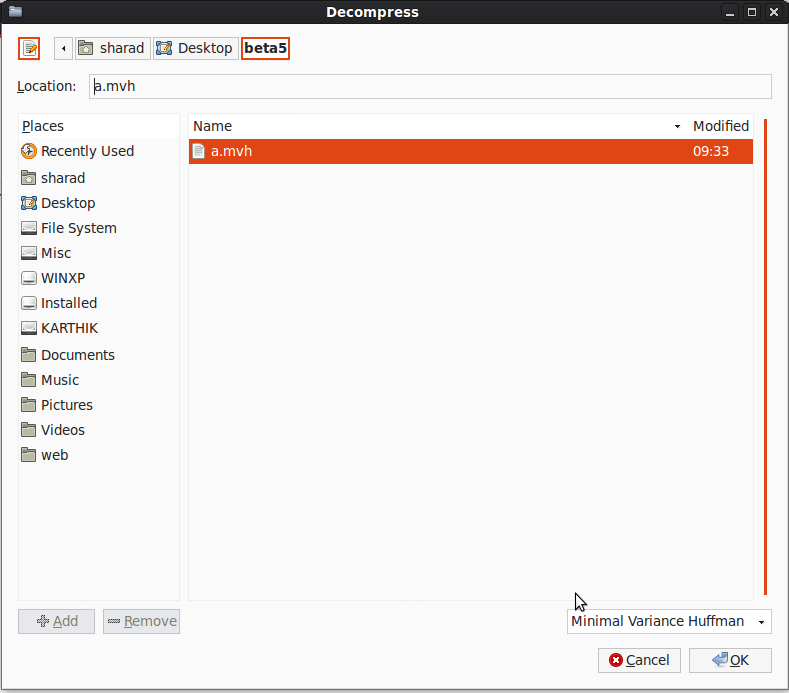
\includegraphics[scale=0.350]{./images/7decselsrc.png}
\end{center}
\caption{Select Decompression Source}
\end{figure}

\begin{figure}[htb]
\begin{center}
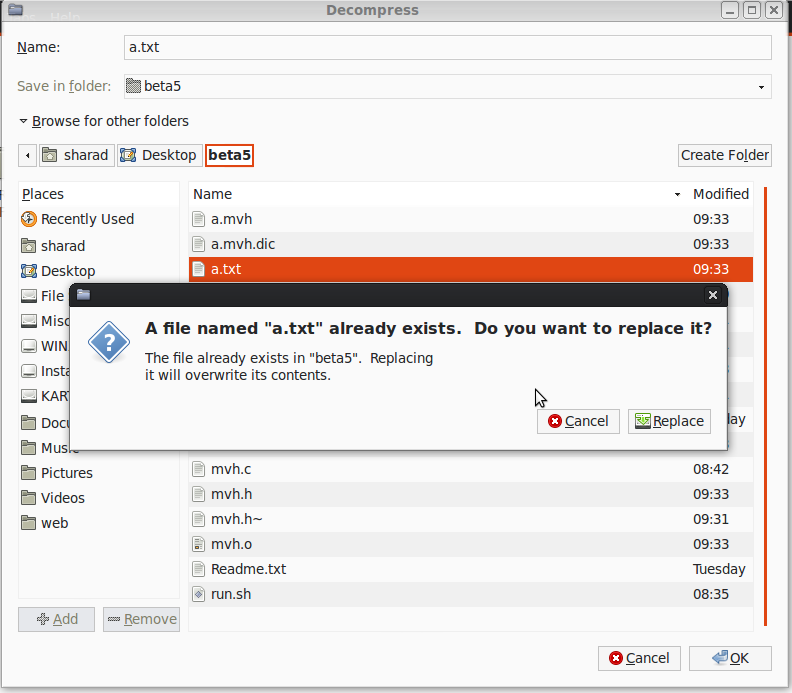
\includegraphics[scale=0.350]{./images/8decseldest.png}
\end{center}
\caption{Select Decompression Destination}
\end{figure}

\begin{figure}[htb]
\begin{center}
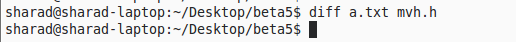
\includegraphics[scale=0.50]{./images/9diff.png}
\end{center}
\caption{Difference between Original and Decompressed Files}
\end{figure}

.
\newpage
.
\newpage
.
\newpage
.
\newpage
.
\newpage

\section{System Testing}
\begin{center}	
\begin{tabular}{|c|c|c|c|}
\hline
File & Original Size & Compressed Size & Ratio \\
\hline
Mvh.h & 4783& 2182 & 33 $\%$\\\hline
Fulla.txt & 271 & 34 & 87  $\%$\\\hline
Folder & 876 & 570 & 34 $\%$\\\hline
Image19.jpg & 40700& 40648 & 0$\%$\\\hline
cs.pdf & 16265 &15973 &  1$\%$\\\hline
Barney.bmp& 1000054& 834136 & 16 $\%$\\\hline
\end{tabular}
\end{center}
\section{Application}
 Arithmetic Coding can be viewed as a generalization of Huffman coding; indeed, in practice arithmetic coding is often preceded by Huffman coding, as it is easier to find an arithmetic code for a binary input than for a nonbinary input. Also, although arithmetic coding offers better compression performance than Huffman coding, Huffman coding is still in wide use because of its simplicity, high speed and lack of encumbrance by patents.

Huffman coding today is often used as a "back-end" to some other compression method.DEFLATE(PKZIP's algorithm) and multimedia codecs such as JPEG and  MP3 have a front-end model and quantisation followed by Huffman coding.
\section{Future Extensions}
Whenever we transfer a text file from the computer to the pendrive,the file should be compressed,and if we click on the compressed file which is present in the pendrive,it should be decompressed to show the original file.

\section{Conclusion}

Minimum variance Huffman Coding is an efficient algorithm for compressing the text files.If the text file contains many repeated sequence of characters or words then a greater compresion is achieved. The compression that was written for a general text file can be modified for a binary file too, so that compression can be done for image files, pdfs, although the compression was not that good enough compared to a text file. Finally minimal variance huffmann tree provides a good compression ratio.

\section{References}
\begin{itemize}
\item Khalid Sayood: Introduction to Data Compression,3rd Edition,Elsevier,2006
\item Wikipaedia : \url{http://en.wikipedia.org/wiki/Huffman_coding}
\end{itemize}

\end{document}
